% \subsection*{Fairness Experiment: Stop, Question, and Frisk data}
A police officer is allowed to stop a person if they have reasonable suspicion that the person has committed, is committing, or is about to commit a crime.
During the stop the officer is allowed to frisk a person (pat-down the person's outer clothing) or search them more carefully.
The stop can result in a summon, an arrest or no further consequences.\par
After a stop was made, the officer is required to fill out a form, documenting the stop. This data is published yearly by the NYPD.
As mentioned in the introduction the so-called "New York strategy" (\cite{gelman2007}) has been criticized for disproportionally targetting African American and Hispanic individuals. This makes the recordings of the stops an interesting resource for fairness research.
It also has been recommended by \cite{Fabris_2022}, not least in the effort to bring more diversity to the datasets used in the field.
For our analysis we are interested in whether a classifier trained to predict the arrest after a stop is discriminatory with respect to race.


\subsection{Setup of the fairness experiment}
We compare the following models in terms of fairness and model performance, measured by the difference in true positive rates (equal opportunity)  and the classification accuracy respectively:
\begin{itemize}
    \item Regular Random Forest
    \item Reweighing to balance disparate impact metric (Pre-Processing)
    \item Classification Fair Logistic Regression With Covariance Constraints Learner (In-Processing)
    \item Equalized Odds Debiasing (Post-Processing)
\end{itemize}
More details about the methods can be found in \cite{mlr3_book}.  
Specifically, for Reweighing, see \href{https://mlr3fairness.mlr-org.com/reference/mlr_pipeops_reweighing.html}{mlr3fairness Reweighing}.  
Refer to \href{https://rdrr.io/cran/mlr3fairness/man/mlr_learners_classif.fairzlrm.html}{Fair Logistic Regression} for more details on the chosen in-processing method.  
For the post-processing strategy, check \href{https://mlr3fairness.mlr-org.com/reference/mlr_pipeops_equalized_odds.html}{Equalized Odds}.  


\subsection{Data description}
\begin{figure}
  \centering
  \begin{minipage}{0.49\textwidth}
      \centering
      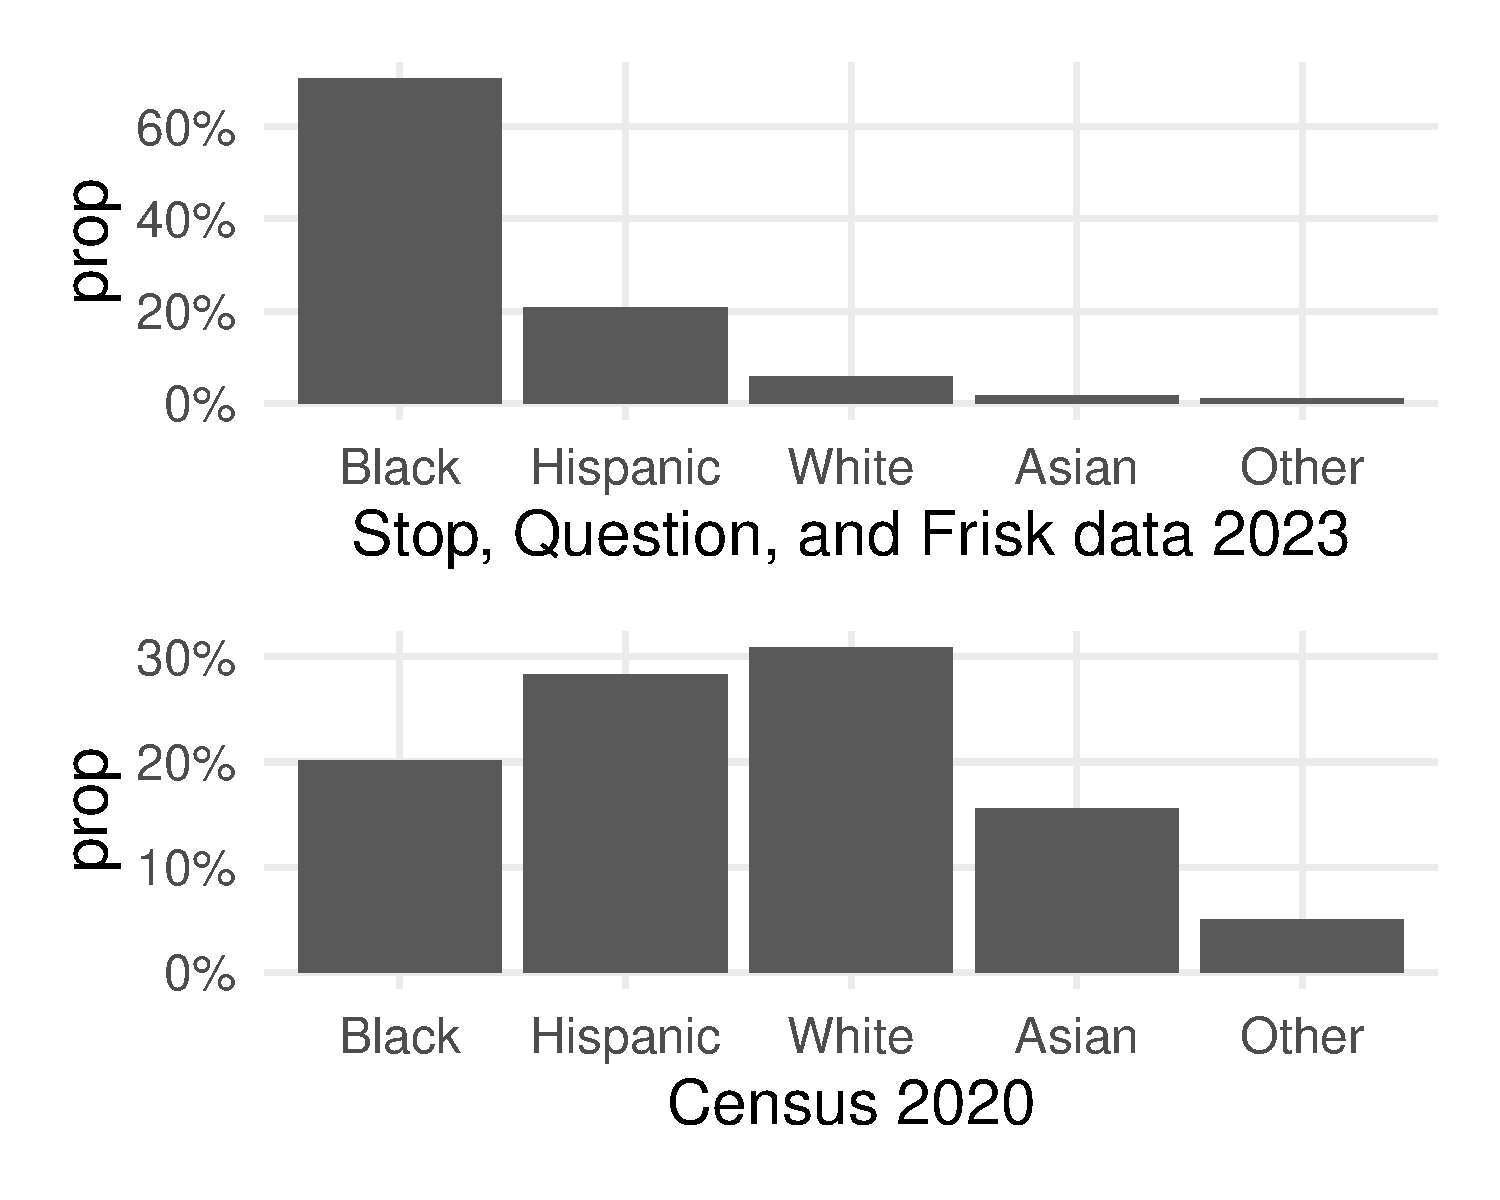
\includegraphics[width=\textwidth]{../figures/sqf_case_study_plot6.pdf}
  \end{minipage}
  \hfill
  \begin{minipage}{0.49\textwidth}
      \centering
      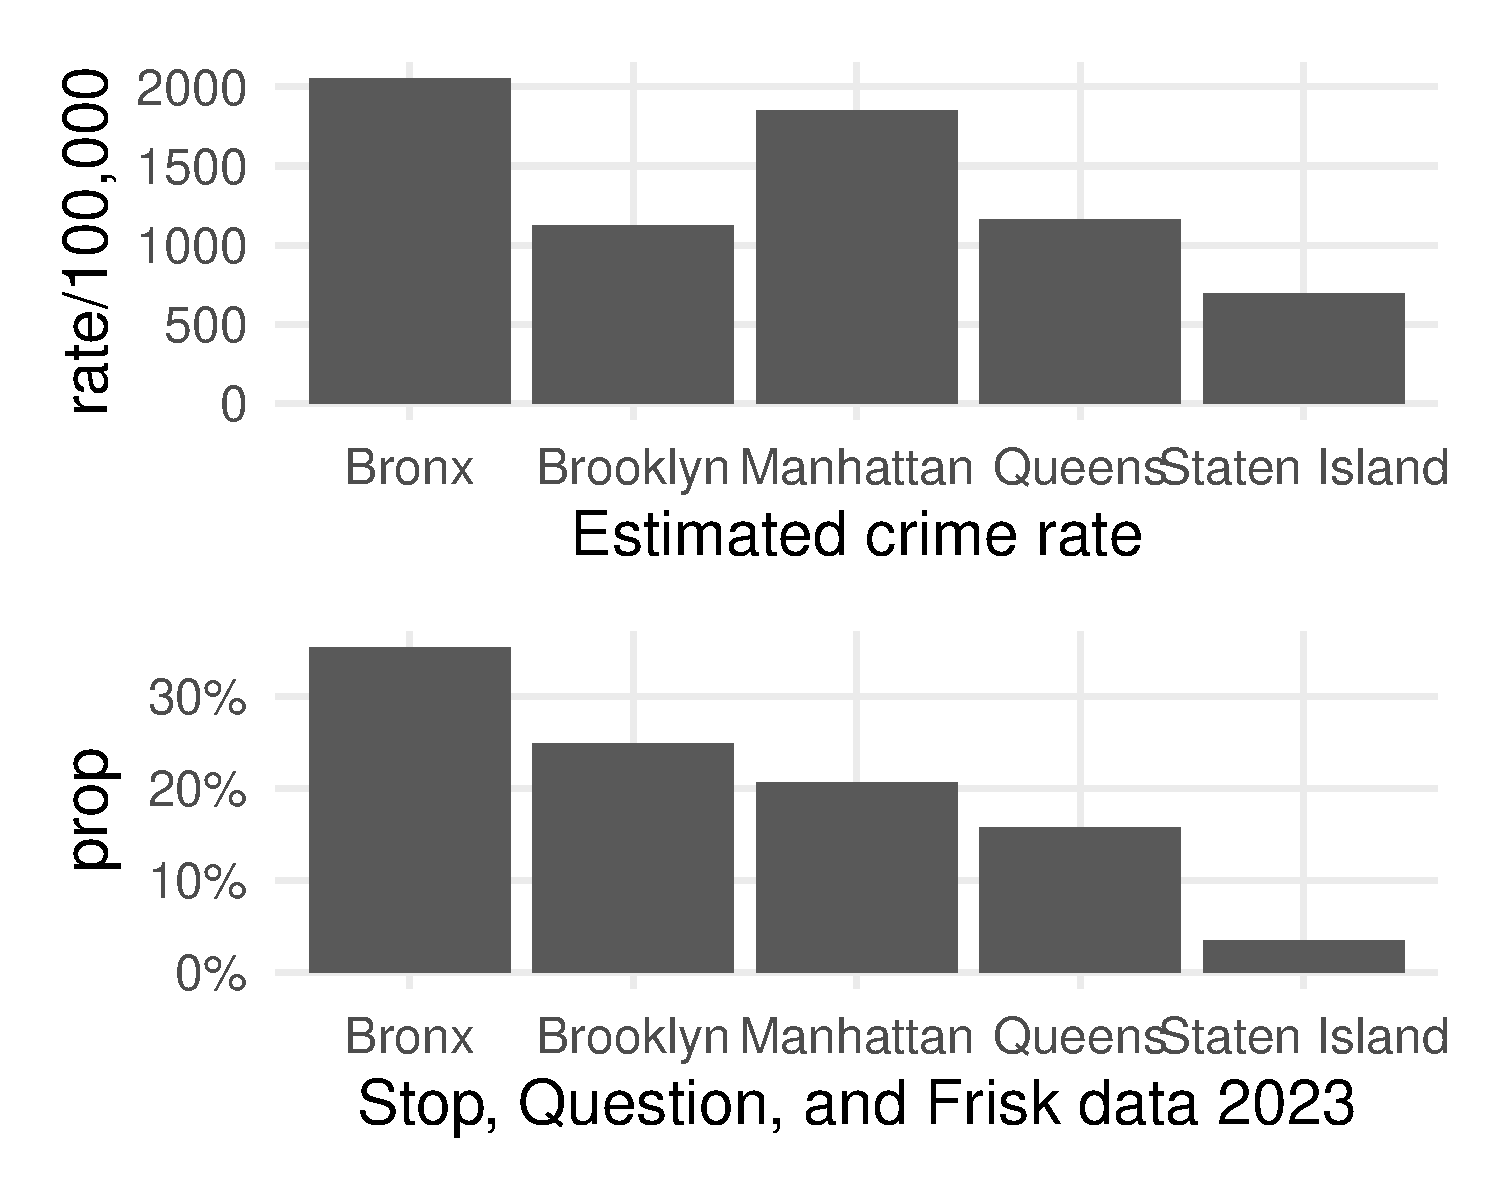
\includegraphics[width=\textwidth]{../figures/sqf_case_study_plot14.pdf}
  \end{minipage}
  \caption{Bar plot comparing the distribution of ethnic groups across boroughs in the SQF 2023 and NYC from 2020 Census (left). On the right a comparison of the estimated borough-wise crime rate per 100,000 citizens with the ethnic distribution of SQF stops.}
  \label{fig:race_distributions}
\end{figure}

As they were the most recent at the time of writing this thesis, we work with the stops from 2023. The raw 2023 dataset consists of 16,971 observations and 82 variables. We first discarded all the variables that have more than 20\% missing values, which leaves 34 variables.
From this reduced dataset we filter out the complete cases and end up with 12,039 observations.\footnote{Simply discarding the missing values and only training on complete cases is discouraged by \cite{fernando2021}. We opt for this approach regardless, since imputation of the missing values is not straight forward
but treating missing values as an extra category will introduce complications when we implement fairness methods.}\par

We summarize "Black Hispanic" and "Black" into the group "Black" and  "American Indian/ Native American" and "Middle Eastern/ Southwest Asian" into the "Other" category. Black people are by far most often stopped, making up 70\% of the total stops; yet, according to 2020 census data black people contribute to only 20\% of the city's population (\autoref{fig:race_distributions}, left). At the same time white people form the majority of New York citizens (30\%) but are involved in merely 6\% of the stops.\par 
After 2012 there has been a stark decline in stops and the police is known to focus their attention on high crime areas. Therefore, we further look at each borough. 
The most stops in 2023 occurred in Bronx and Brooklyn. Based on report of the NYPD and population statistics from 2020, the Bronx also has the highest estimated crime rate per 100,000 citizens. Manhattan has a similarly high crime rate, but fewer stops. Note that Bronx and Brooklyn happen to be the boroughs with the highest proportion of black citizens (\autoref{fig:race_distributions}, right).\par

After a more general overview of the dataset, we turn to the outcome of interest. In the cleaned 2023 data about 31\% of stops result in an arrest.
\autoref{tab:groupwise_arrestment_rates_2023} shows that the disparities in arrestment across ethnic groups is in general low.
% \autoref{fig:arrestment_rates_clean_data}.
As group fairness metrics are observational and constructed from the joint probability of $Y, \hat{Y}, A$, this already gives us a hint that the classifier trained to predict the arrestment of a suspect might show little racial disparities.

\afterpage{
    \begin{table}[!h]
        \centering
        \begin{minipage}{0.48\linewidth}
            \centering
            \begin{tabular}{|ll|}
                \hline
                Group & Prop \\ 
                \hline
                Black & 30.56\% \\ 
                Hispanic & 31.60\% \\ 
                White & 37.95\% \\ 
                Asian & 37.84\% \\ 
                Other & 31.45\% \\ 
                \hline
            \end{tabular}
            \caption{Group-wise arrestment rates in 2023} 
            \label{tab:groupwise_arrestment_rates_2023}
        \end{minipage}
        \hfill
        \begin{minipage}{0.48\linewidth}
            \centering
            \begin{tabular}{|ll|}
                \hline
                Group & Prop \\ 
                \hline
                Black & 5.988\% \\ 
                Hispanic & 5.830\% \\ 
                White & 6.859\% \\ 
                Asian & 5.840\% \\ 
                Other & 4.575\% \\ 
                \hline
            \end{tabular}
            \caption{Group-wise arrestment rates in 2011} 
            \label{tab:groupwise_arrestment_rates_2011}
        \end{minipage}
    \end{table}
}

Given the evolution of stops over the years and the 2013 ruling, the question arises whether a classifier trained on data from the unconstitutional period (2004-2012) will perform differently.
For a comparison, we therefore train an additional random forest classifier on data from 2011. This is the year with the most stops. We carry out the same data cleaning steps, starting with 685,724 recorded stops and reducing this to 651,567 clean observations. Note that these are around 40 times more stops than in 2023.
This means that the 2011 data has substantially more low-risk stops; only around 6\% result in an arrest. This is a stark contrast to the 31\% in 2023. As seen in \autoref{tab:groupwise_arrestment_rates_2011} the differences in arrestment rate across ethnic groups are minor. As in 2023 white people have the highest arrestment rate.\par
We select features that reflect the information available to the officer at the time of the arrest decision. This includes details about the stop's progression, such as whether the person was frisked or issued a summon. We consider these outcomes as intermediate steps before an arrest. Additionally, we control for factors like the time of the stop and whether the officer was in uniform. This feature selection is inspired by \cite{Badr2022DTFANSP}.

\subsection{Results of the fairness experiment}
For the training of the classifiers, we dichotomize the race attribute by grouping "Black" and "Hispanic" as people of colour ("PoC") and "White", "Asian", and "Other" as white ("White"). We run a five-fold cross validation and show the results in \autoref{fig:fairness_experiment}.\par
\begin{figure}[ht]
    \centering
    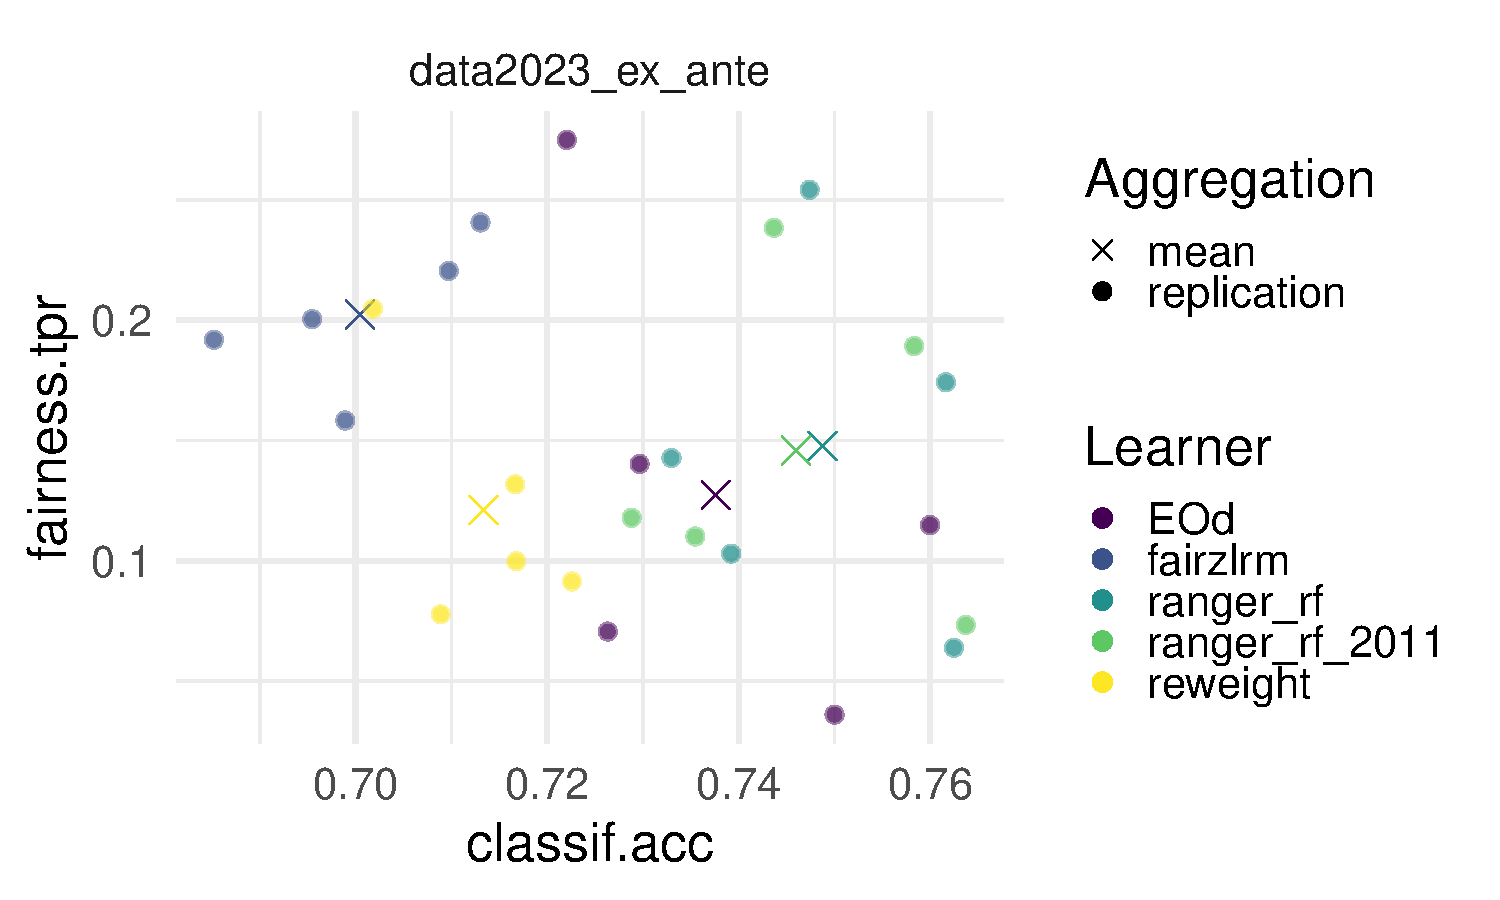
\includegraphics[width=0.7\textwidth]{../figures/sqf_case_study_plot3.pdf}
    \caption{Comparison of learners with respect to classification accuracy (x-axis) and equal opportunity (y-axis) across (dots) and aggregated over (crosses) five folds.}
    \label{fig:fairness_experiment}
\end{figure}
The x-axis shows the learner's accuracy and on the y-axis we plot the absolute difference in true positive rates across groups. In the bottom right corner we find fair and accurate classifiers. In terms of fairness reweighing and the equalized odds post-processing method perform best. However, the regular random forest classifier comes close to their fairness performance and performs slightly more accurate. Surprisingly, it does not make any difference for the fairness if the classifier is trained on 2011 or 2023 data.
We examined the model closer and find that due to the low prevalence in the population, a classifier trained on 2011 data primarily suffers from the highly skewed distribution of arrests. The classifier largely predicts the negative label for \textit{anyone} regardless of race, which overshadows potential fairness concerns.
The fairness adjusted logistic regression performs worst in terms of accuracy and fairness.
As the picture could change depending on the chosen fairness metric (y-axis), we also experimented with other metrics, such as equalized odds or predictive parity. In all cases the regular random forest does not perform worse in terms of fairness but better in terms of accuracy than most fairness adjusted classifiers.




Since the classifiers perform similarly, we choose the regular random forest trained on 2023 to examine the model closer.
In \autoref{fig:fairness_density} on the left we plot the prediction score densities for each group. We can see that in general white people tend to have higher predicted probabilities than PoC. The mode for the scores for non-white individuals is around 0.05 while it is around 0.125 for white individuals. The score resembles the probability of being predicted positive (arrested). This may suggest that PoC are involved in more low-risk stops than white suspects. In \autoref{fig:fairness_density} on the right we plot the absolute difference in selected group fairness metrics.
Exact equality of the group fairness metrics cannot be expected in practice, so it is common to allow for a margin of error $\epsilon$. Taking $\epsilon = 0.05$, the classifier is fair according to each of the selected metrics, though the difference in positive predictive rates is close to 0.05.\par
\begin{figure}[htbp]
    \centering
    \begin{minipage}{0.49\textwidth}
        \centering
        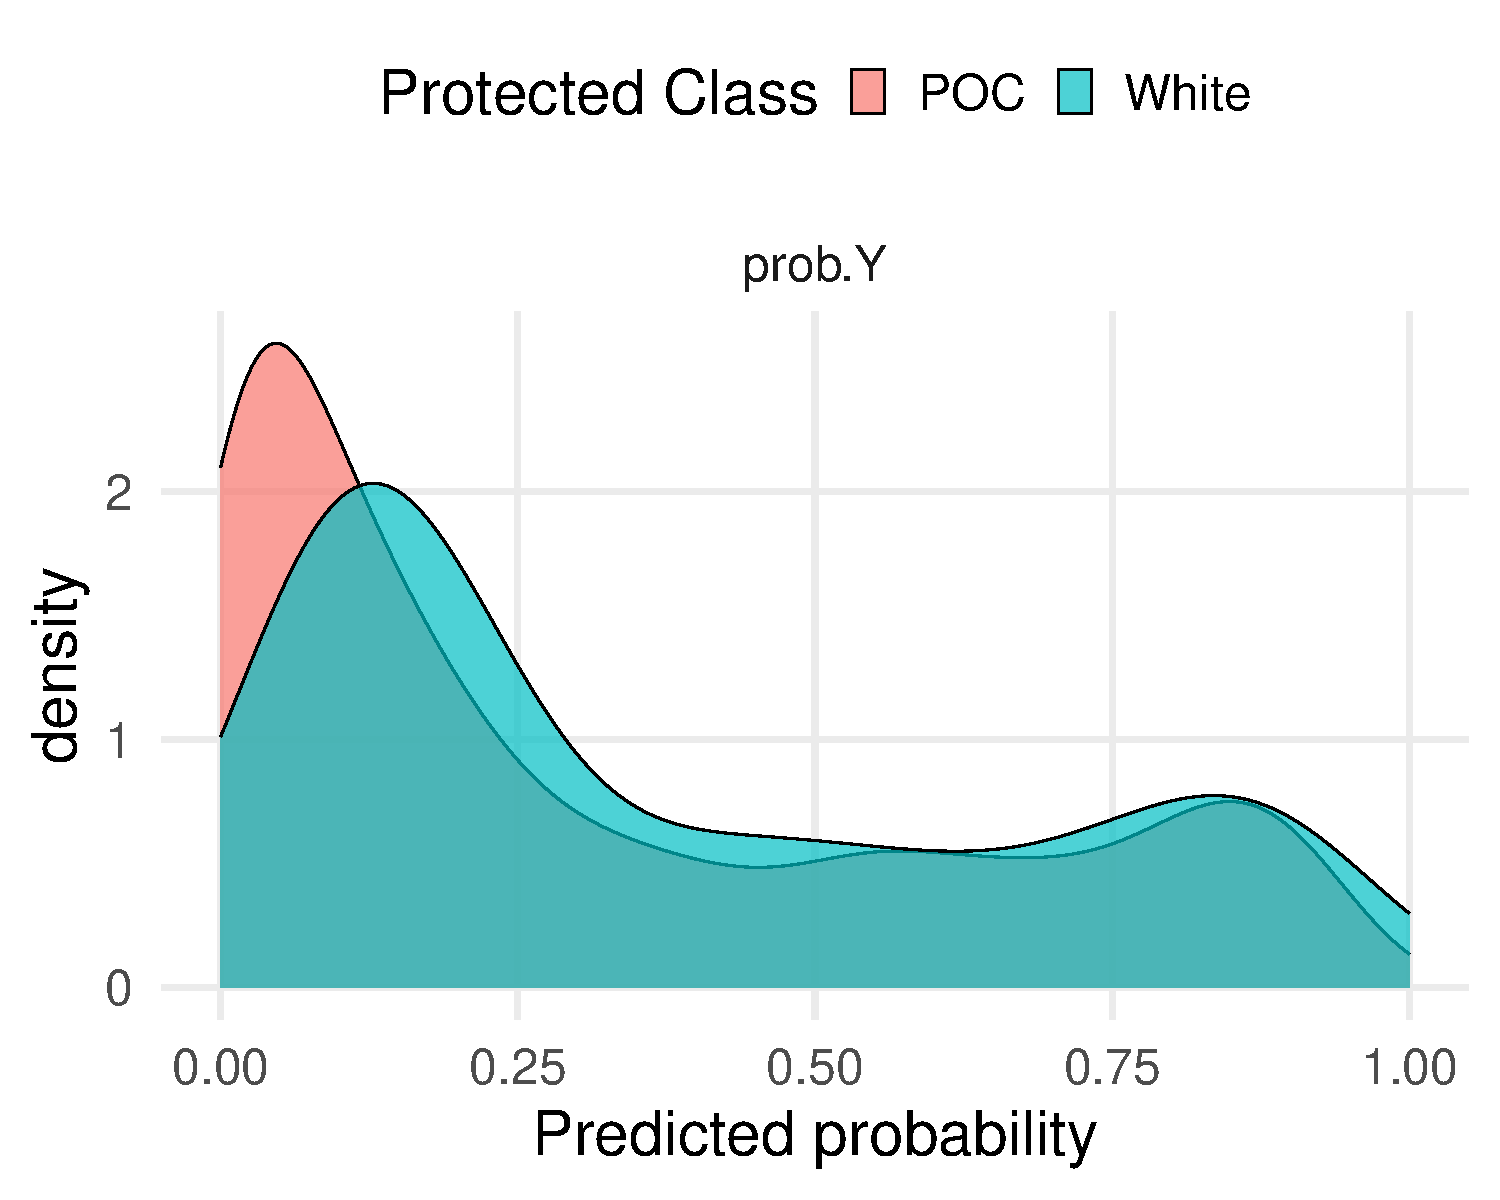
\includegraphics[width=\textwidth]{../figures/sqf_case_study_plot1.pdf}
    \end{minipage}
    \hfill
    \begin{minipage}{0.49\textwidth}
        \centering
        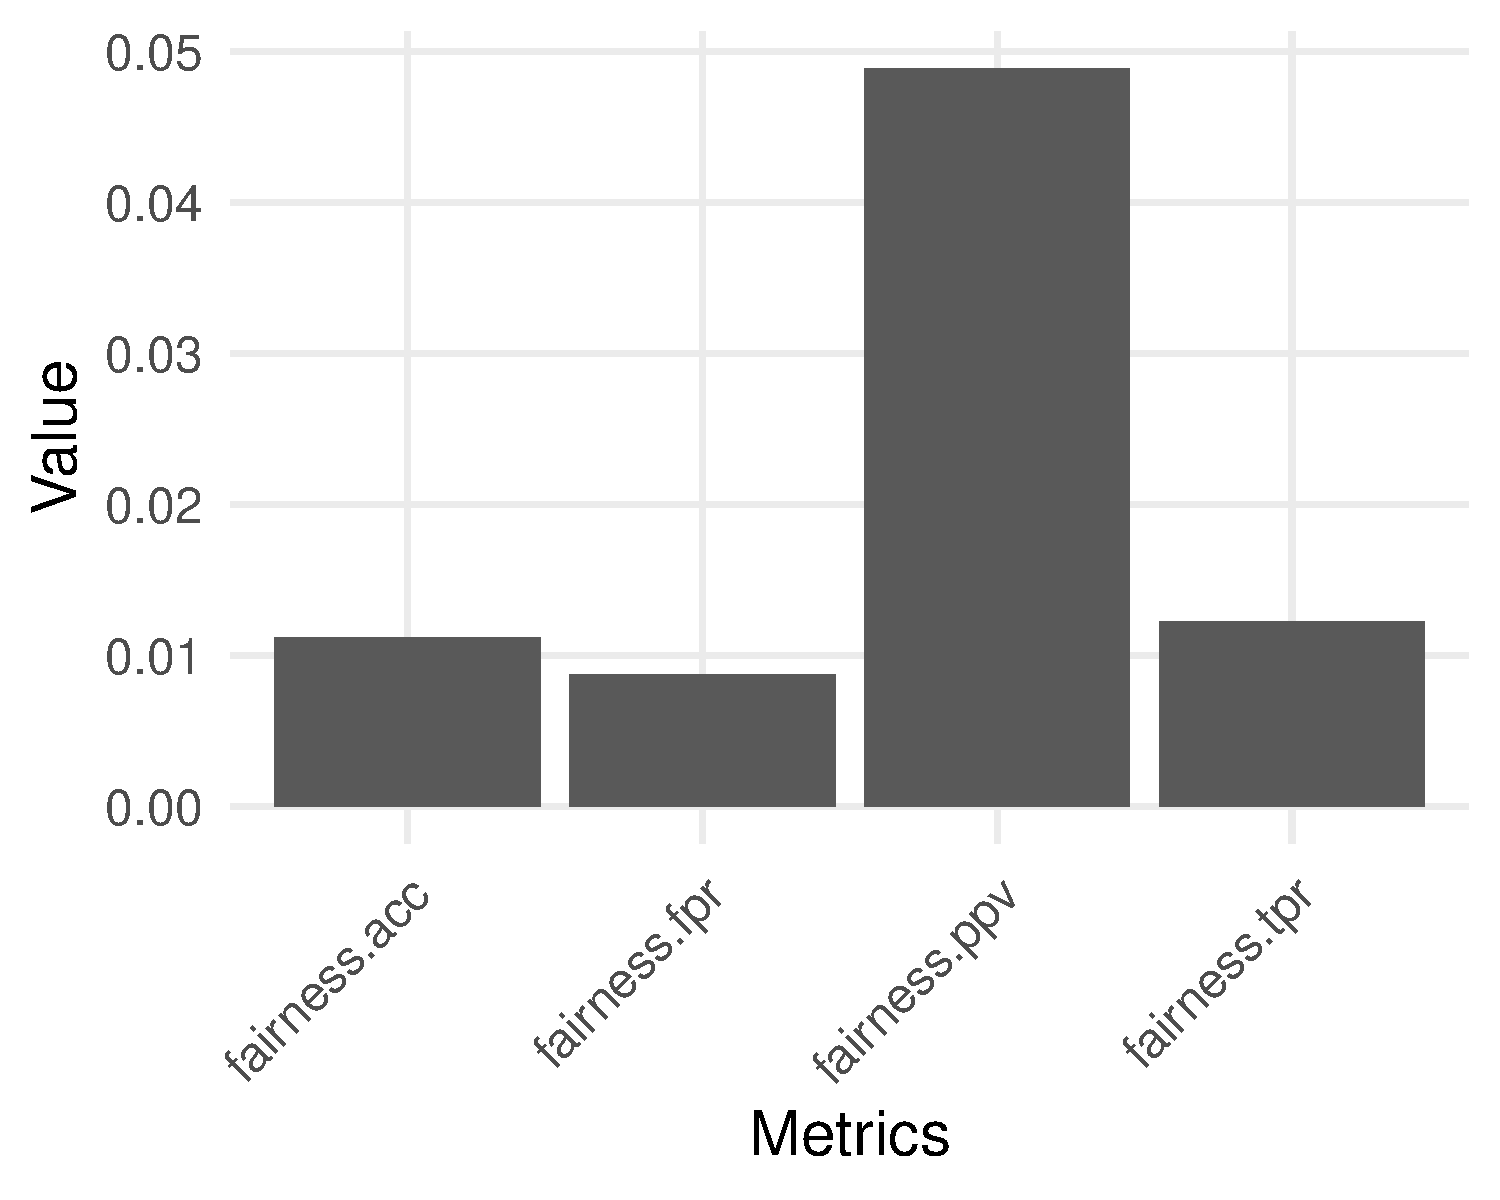
\includegraphics[width=\textwidth]{../figures/sqf_case_study_plot2.pdf}
    \end{minipage}
    \caption{Fairness prediction density plot (left) showing the density of predictions for the positive class split by "PoC" and "White" individuals. The metrics comparison barplot (right) displays the model's absolute differences across the specified metrics.}
    \label{fig:fairness_density}
\end{figure}


For a more nuanced picture, we additionally report the group-wise error metrics in \autoref{tab:groupwise_metrics_2023}.
As the absolute differences in the plots have already shown, the \textit{separation} metrics are virtually the same across groups. For the \textit{sufficiency} metrics, the positive predictive value is slightly higher for white individuals, meaning a positive prediction is more likely to be correct for them than for PoC. Conversely, the negative predictive value is higher for PoC, indicating that a negative prediction is more likely to be correct for them than for white individuals.

\begin{table}[htbp]
    \centering
    \begin{tabular}{|rrrrrrr|}
      \hline
     & TPR & FPR & NPV & PPV & FDR & Acc \\ 
      \hline
      PoC & 0.75 & 0.07 & 0.89 & 0.84 & 0.16 & 0.88 \\ 
      White & 0.74 & 0.06 & 0.85 & 0.89 & 0.11 & 0.86 \\ 
       \hline
    \end{tabular}
    \caption{Group fairness metrics for RF classifier trained on 2023 SQF data.} 
    \label{tab:groupwise_metrics_2023}
\end{table}

In general, it seems like the classifier trained on SQF data to predict the arrest of a suspect is not discriminatory against PoC. In contrast, it even performs slightly better for PoC than for white people on many of the common performance metrics. \cite{Badr2022DTFANSP} have similar findings.\par

In their study they chose six representative machine learning algorithms (Logistic Regression, Random Forest, Extreme Gradient Boost, Gaussian Naïve Bayes, Support Vector Classifier) to predict the arrest of a suspect. Fairness is measured with six different metrics (Balanced Accuracy, Statistical Parity, Equal Opportunity, Disparate Impact, Avg. Odds Difference, Theil Index) and separate analysis are conducted with sex and race as PA.
They compare the fairness of the regular learner to the fairness of learner with a pre-processing method (reweighing) and a post-processing method (Reject Option-based Classifier).
All in all, they find that the regular models to not perform worse in terms of fairness than the fairness adjusted models. This leads them to conclude "[...] that there is no-to-less racial bias that is present in the NYPD Stop-and-Frisk dataset concerning coloured and Hispanic individuals."\par
What both of our case studies have in common is that the models were trained on recent data and select arrest as target. We trained our model on 2023 stops and \cite{Badr2022DTFANSP} used 2019 stops. The authors specifically identified time as an important factor in their results and state: "The NYPD has taken crucial steps over the past years and significantly reduced racial- and [gender-based] bias in the stops leading to arrests. This conclusion nullifies the common belief that the NYPD Stop-and-Frisk program is biased toward [coloured] and Hispanic individuals." Is this the whole picture?



  


